\documentclass[final]{fhnwreport}         %[mode] = draft or final
%%---Main Packages-----------------------------------------------------------------------
\usepackage[english, ngerman]{babel}	%Mul­tilin­gual sup­port for LaTeX
\usepackage[T1]{fontenc}				      %Stan­dard pack­age for se­lect­ing font en­cod­ings
\usepackage[utf8]{inputenc}				  %Ac­cept dif­fer­ent in­put en­cod­ings
\usepackage{lmodern}                 %The newer Font-Set
\usepackage{textcomp}					      %LaTeX sup­port for the Text Com­pan­ion fonts
\usepackage{graphicx} 					      %En­hanced sup­port for graph­ics
\usepackage{float}						        %Im­proved in­ter­face for float­ing ob­jects
%\usepackage{ifdraft}                %Let you check if the doc is in draft mode

%%---Useful Packages---------------------------------------------------------------------
\usepackage[pdftex,dvipsnames,tables]{xcolor}  %Driver-in­de­pen­dent color ex­ten­sions for LaTeX
\usepackage{csquotes}                %Simpler quoting with \enquote{}
\usepackage{siunitx} 					      %A com­pre­hen­sive (SI) units pack­age
\usepackage{listings}					      %Type­set source code list­ings us­ing LaTeX
\usepackage[bottom]{footmisc}			  %A range of foot­note op­tions
\usepackage{footnote}					      %Im­prove on LaTeX's foot­note han­dling
\usepackage{verbatim}					      %Reim­ple­men­ta­tion of and ex­ten­sions to LaTeX ver­ba­tim
\usepackage[textsize=footnotesize]{todonotes} %Mark­ing things to do in a LaTeX doc­u­ment
\usepackage{lipsum}              % Gives you access to blindtext

%%---Tikz Packages-----------------------------------------------------------------------
%\usepackage{standalone}
%\usepackage{tikz}
%\usepackage{circuitikz}
%\usetikzlibrary{arrows}
%\usetikzlibrary{calc}
%\usetikzlibrary{intersections}

%%---Math Packages-----------------------------------------------------------------------
\usepackage{amsmath}					    %AMS math­e­mat­i­cal fa­cil­i­ties for LaTeX
%\usepackage{amssymb}					  %Type­set­ting symbols (AMS style)
%\usepackage{array}						  %Ex­tend­ing the ar­ray and tab­u­lar en­vi­ron­ments
%\usepackage{amsthm}					    %Type­set­ting the­o­rems (AMS style)

%%---Table Packages----------------------------------------------------------------------
\usepackage{tabularx}					  %Tab­u­lars with ad­justable-width columns
%\usepackage{longtable}
\usepackage{multirow}					  %Create tab­u­lar cells span­ning mul­ti­ple rows
\usepackage{multicol}					  %In­ter­mix sin­gle and mul­ti­ple columns

%%---PDF / Figure Packages---------------------------------------------------------------
\usepackage{pdfpages}					  %In­clude PDF doc­u­ments in LaTeX
\usepackage{pdflscape}					  %Make land­scape pages dis­play as land­scape
%\usepackage{subfig}					    %Fig­ures di­vided into sub­fig­ures

%%---Other Packages----------------------------------------------------------------------
%\usepackage{xargs}              %De­fine com­mands with many op­tional ar­gu­ments


%%---Main Settings-----------------------------------------------------------------------
\graphicspath{{./graphics/}}			%Defines the graphicspath
%\geometry{twoside=false}				%twoside=false disables the "bookstyle"
\setlength{\marginparwidth}{2cm}
\overfullrule=5em						    %Creates a black rule if text goes over the margins => debugging

%%---User Definitions--------------------------------------------------------------------
%%Tabel-Definitions: (requires \usepackage{tabularx})
\newcolumntype{L}[1]{>{\raggedright\arraybackslash}p{#1}}    %column-width and alignment
\newcolumntype{C}[1]{>{\centering\arraybackslash}p{#1}}
\newcolumntype{R}[1]{>{\raggedleft\arraybackslash}p{#1}}					                        %loads all packages, definitions and settings	

\usepackage[style=ieee,urldate=comp,backend=biber]{biblatex}
%\usepackage[style=apa,urldate=comp,backend=biber]{biblatex}
\addbibresource{literature/beispiel_bib.bib}
											
\title{Cloudbasiertes Praxisrufsystem}  %Project Title
\author{IP 5}                      %Document Type => Technical Report, ...

\begin{document}

%%---TITLEPAGE---------------------------------------------------------------------------
\selectlanguage{ngerman} %ngerman or english
\maketitle

\begin{figure}[H]
\centering

\includegraphics[width=\linewidth]{wip.png}
\end{figure}

\vfill

\begin{center}
\renewcommand\arraystretch{2}
\begin{tabular}{>{\bf}p{4cm} l}
Studenten & Joshua Villing, Kevin Zellweger\\
Fachbetreuer & Daniel Jossen\\
Auftraggeberin & Daniel Jossen\\
Studiengang & Informatik\\
Hochschule & Hochschule für Technik
\end{tabular}
\end{center}

\clearpage
			
%%---ABSTRACT----------------------------------------------------------------------------
\selectlanguage{ngerman}				%ngerman or english
\thispagestyle{empty}
\begin{abstract}
Das Abstract ist eine Art Zusammenfassung des ganzen Dokuments. Es gibt einen Einblick in die Aufgabenstellung, wie diese umgesetzt wurde und welches Ergebnis erreicht wurde. Aus diesem Grund wird das Abstract immer ganz am Schluss der Arbeit verfasst. Es besteht aus einem zusammengehörenden Absatz und umfasst ungefähr 10 bis 20 Zeilen.
Formeln, Referenzen oder andere Unterbrechungen haben im Text nichts zu suchen.
Direkt unter dem Abstract folgt eine Liste von drei bis vier Stichworten/Keywords. Diese werden in alphabetischer Reihenfolge aufgelistet und beschreiben das Themengebiet der Arbeit.

\vspace{2ex}

\textbf{Keywords: Anleitung, LaTeX, Thesis, Vorlage}

\vspace{2ex}

\textbf{Management Summary} siehe PF-IK.

\end{abstract}	

\clearpage

\section*{Vorwort}

\lipsum[1-2]

Fakultativ, siehe PF-IK (URL)


%%---TABLE OF CONTENTS-------------------------------------------------------------------
\pagenumbering{Roman}		
\selectlanguage{ngerman}				%ngerman or english
\tableofcontents
\clearpage

%%---TEXT--------------------------------------------------------------------------------
\pagenumbering{arabic}
\section{Proof Of Concept}



\subsection{Anforderungen}

\begin{itemize}
    \item  Als <Sender Rolle> möchte ich Notifikationen versenden können. 
    \item Als <Empfänger Rolle> möchte ich Notifikationen in der Applikation sehen, wenn die Applikation geöffnet ist.  
    \item Als <Empfänger Rolle> möchte ich Notifikationen über das OS erhalten, wenn die Applikation minimiert ist. 
\end{itemize}

\subsection{Restriktionen}

\begin{itemize}
    \item Nur 1 Client. 
    \item Nur 1 fixe Notifikation. Keine Types. 
    \item Notifikation wird vom Client gesendet und vom selben Client empfangen. 
    \item Keine Authentication oder Authorization. 
  
\end{itemize}



\subsection{Architektur}


\subsection{Messaging Service}



\subsubsection{Überblick}

Für den Proof Of Concept wird eine vereinfachte Architektur aufgebaut. Für den Proof Of Concept sehen wir drei Applikationen vor: 

\begin{itemize}
    \item Messaging Service
    \item Cloud Service
    \item Mobile Client
\end{itemize}


\begin{figure}[H]
\centering
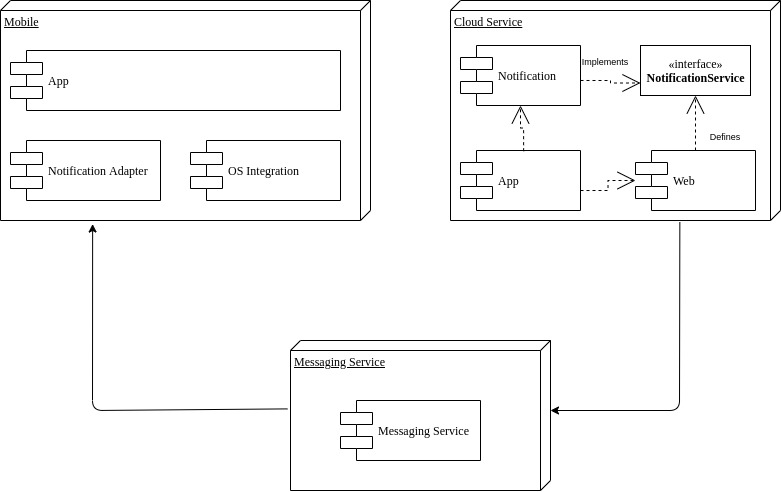
\includegraphics[width=\linewidth]{IP5_POC_Cloud_Architecture.jpg}
\end{figure}




\subsection{Messaging Service}

Dies wird ein externer Service den wir in die Applikationen einbinden. Standard hierfür ist Firebase Notifications. 

Der Messaging Service nimmt Notifikationen vom Cloud Service entgegen und gibt diese an den Mobile Client wieder. 

Dafür müssen auf beiden Seiten Komponenten eingebaut werden, die mit dem Messaging Service kommunizieren. 



\subsection{Cloud Service}

Der Cloud Service für den POC ist in drei Module unterteilt: 

App - Dieses Modul fasst die anderen Module zusammen und bietet die Funktionalität den Service zu starten. Im Build Prozess es dieses Modul, dass am Ende das deploybare Artifakt liefert. 

Web - Dieses Modul bietet eine REST SChnittstelle nach aussen die von einem Client angesprochen werden kann. Diese Schnittstelle bietet die Möglichkeit eine Notification zu senden. Dazu definiert das Web Modul ein Interface "NotificationService"

Notification - Dieses Modul implementiert das NotificationService Interface aus dem Web Modul. In der Implementation wird die Integration an den Message Service implementiert. 




\subsection{Mobile Client}

Der Mobile Client implementiert die Anbindung an den Messaging Service. 

Als Reaktion auf eine Notification wird eine OS Push Notifikation gesendet. 

Als Reaktion auf eine Notification wird eine Rückmeldung im UI angezeigt. 

Das UI bietet einen Button der eine Anfrage an die REST Schnittstelle im Cloud Service sendet. 



\clearpage

\section{Einleitung}

\lipsum[3-4]

Einleitungsbeispiele siehe PF-IK (URL)
\section{Grundlagen, Stand der Forschung}

\emph{Leseführung.} \lipsum[6-6]

Ein bestimmtes Paper: \cite{h_schmid_approximating_2000}. Und noch aschnell die ganze Bibliographie zitieren: \cite{*}.

\subsection{Theorie 1}

\emph{Informieren und orientieren.} Das Schema in Abbildung~\ref{fig:software_struktur} enthält \ldots, \lipsum[7-7]

\begin{figure}[b]
\begin{center}
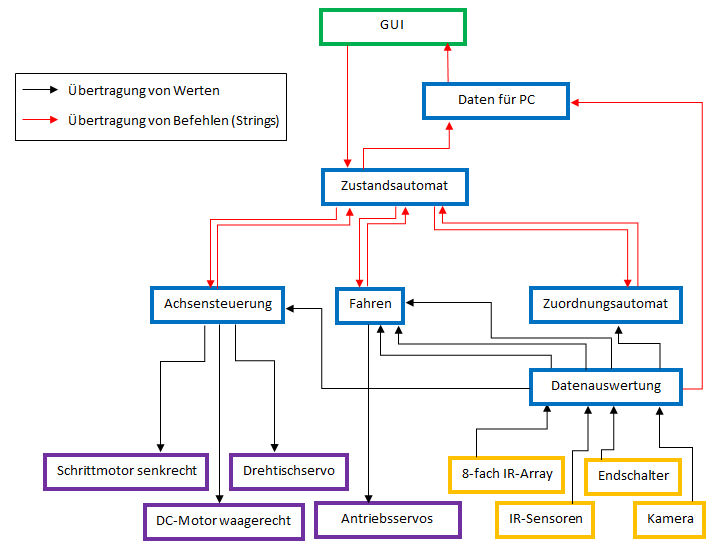
\includegraphics[width=\linewidth]{graphics/software_struktur.png}
\end{center}
\caption{Realisierte Software-Struktur in LABView}
\label{fig:software_struktur}
\end{figure}

\subsection{Unterkapitel}

Ein Beispiel für die Darstellung von Formeln. Aus den nachfolgenden zwei Formeln ist ersichtlich, dass sie das gleiche Verhältnis zwischen den Quadraten der drei Seiten eines rechtwinkligen Dreiecks darstellen, wobei $a$ und $b$ für die Längen der beiden Katheten und $c$ für die Länge der Hypotenuse steht. Aus dem Satz des Pythagoras,
\begin{equation}
a^2+b^2=c^2\;,
\end{equation}
lässt sich mit Hilfe einer einfachen Umformung das Quadrat der einen Kathete des rechtwinkligen Dreiecks aus den Quadraten der anderen beiden Seitenlän-gen herleiten:
\begin{equation}
a^2=c^2-b^2\;.
\end{equation}

Durch eine andere Umformung erhält man auch das Quadrat der anderen Kathete:
\begin{equation}
b^2=c^2-a^2\;.
\end{equation}

Wie die Formeln in Word korrekt zu formatieren und die Nummerierung am rechten Seitenrand zu platzieren sind, ist den Videos auf der PF-IK zu entnehmen. \LaTeX macht das automatisch für Sie.

\section{Kapitel This}
Eins, Zwei, Test, Eins, Zwei.

\lipsum[8-8]

\subsection{Untertitel 1}

\lipsum[9-10]

\subsection{Untertitel 2}

\lipsum[11-13]

\subsubsection{Untertitel 3.~Grades}

Tabelle~\ref{tab:beispieltabelle} zeigt \ldots\;. \lipsum[14-14]

\begin{table}
  \begin{center}
    \begin{tabular}{l|S|r}
      \textbf{Value 1} & \textbf{Value 2} & \textbf{Value 3}\\
      $\alpha$ & $\beta$ & $\gamma$ \\
      \hline
      \multirow{2}{*}{12} & 1110.1 & a\\ % <-- Combining 2 rows with arbitrary with (*) and content 12
      & 10.1 & b\\ % <-- Content of first column omitted.
      \hline
      3 & 23.113231 & c\\
      4 & 25.113231 & d\\
    \end{tabular}
  \end{center}
  \caption{Beispieltabelle, übernommen von \url{https://www.latex-tutorial.com/tutorials/tables/}.}
  \label{tab:beispieltabelle}
\end{table}

\lipsum[15-15]

\subsubsection{Untertitel 3.~Grades}

\lipsum[16-17]
\section{Kapitel That}

\lipsum[42-42]

\subsection{Code-Beispiel}

\lipsum[43-43]

\lstdefinestyle{custompython}{
  belowcaptionskip=1\baselineskip,
  breaklines=true,
  frame=L,
  xleftmargin=\parindent,
  numbers=left,
  language=Python,
  showstringspaces=false,
  basicstyle=\footnotesize\ttfamily,
  keywordstyle=\bfseries\color{green!40!black},
  commentstyle=\itshape\color{purple!40!black},
  identifierstyle=\color{blue},
  stringstyle=\color{orange},
}

\lstinputlisting[caption=Ein längeres Codebeispiel in der Programmiersprache Python, style=custompython]{listings/python_example.py}


%%---BIBLIOGRAPHY------------------------------------------------------------------------
{\sloppypar
\printbibliography[heading=bibintoc]
}

%%---APPENDIX----------------------------------------------------------------------------
\begin{appendix} %Anhang
\section{Ein Anhang}

\lipsum[61-64]

%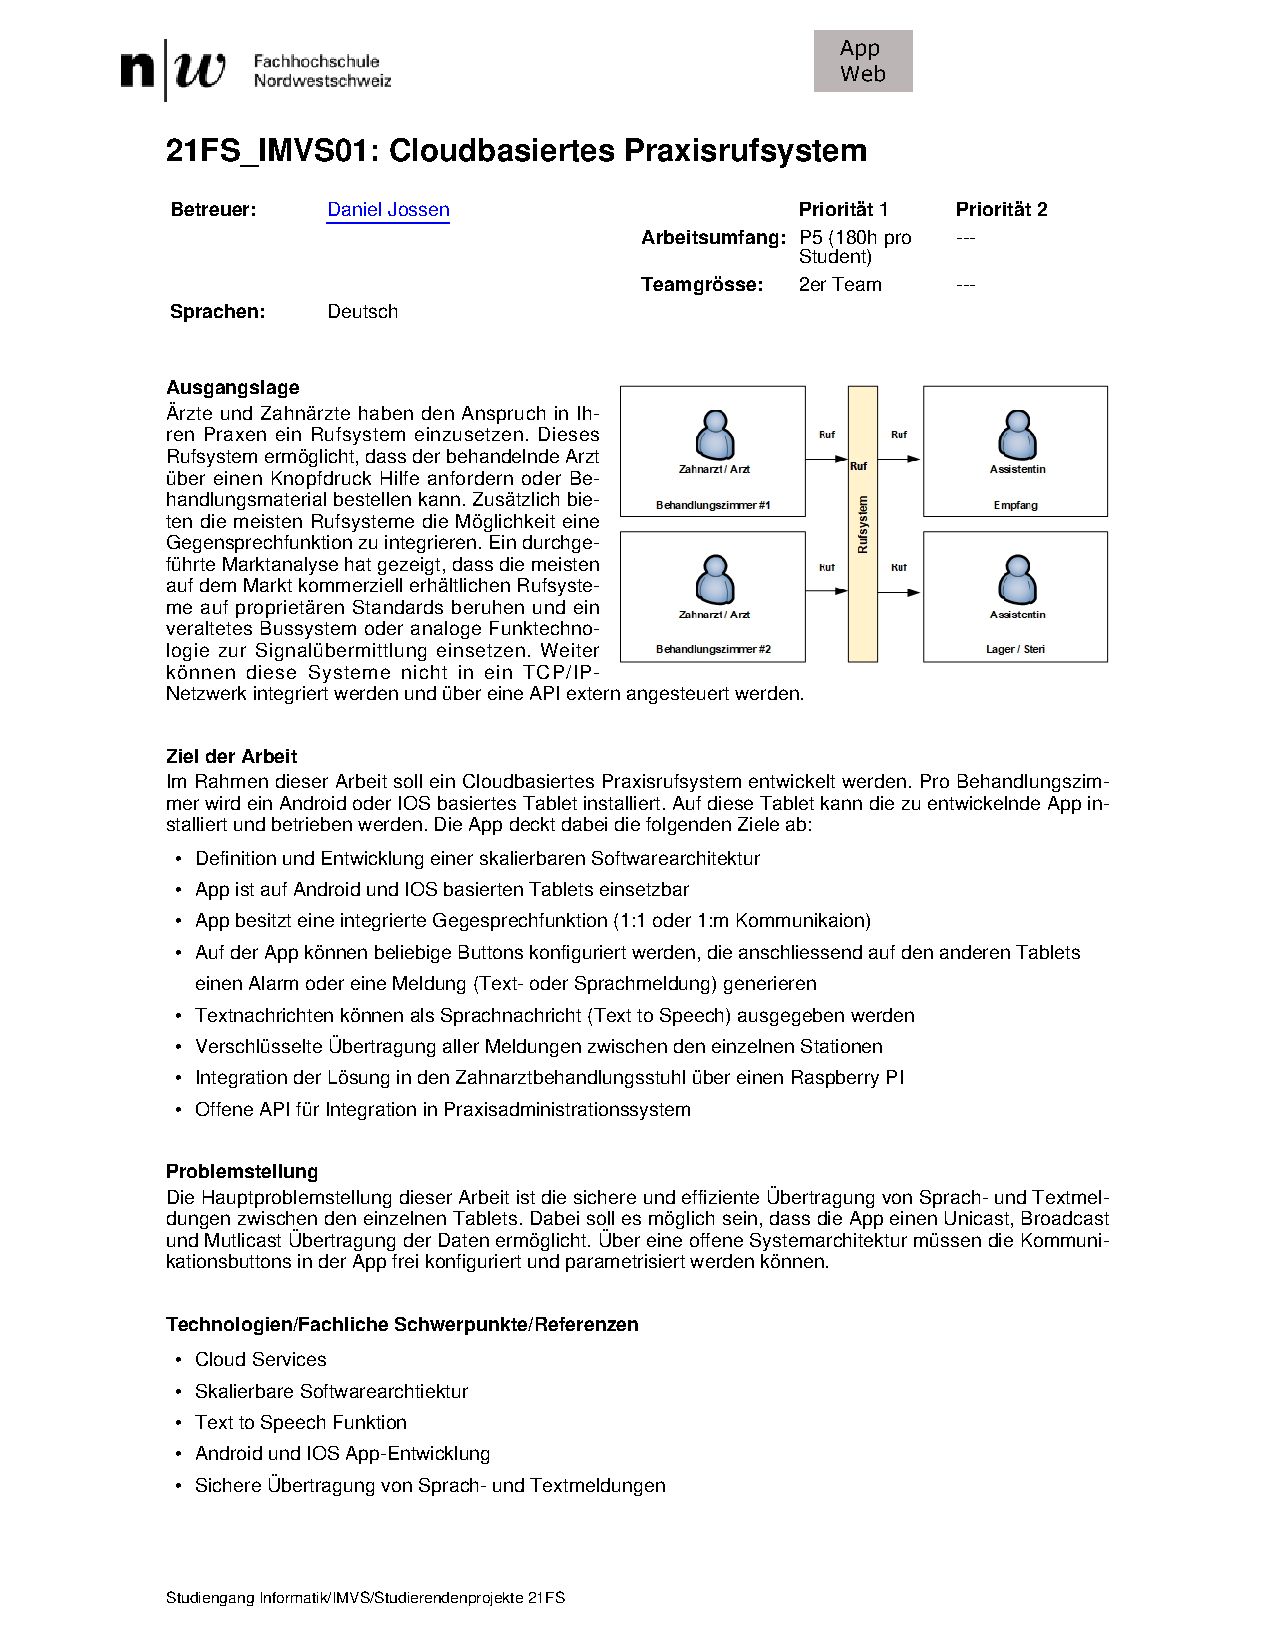
\includepdf[pages={1-2},nup=1x2,landscape=true,scale=0.85,offset=10 -40,pagecommand={\section{Eingefügtes Dokument; zwei Seiten auf einer}\label{app:Aufgabenstellung}\thispagestyle{myheadings}}]{appendix/aufgabenstellung.pdf} \newpage

%%Bei mehrseitigen Dokumenten die folgenden Seiten ohne Überschrift:
%\includepdf[pages={3-6},nup=1x2,landscape=true,scale=0.85,offset=10 -40,pagecommand={\thispagestyle{myheadings}}]{appendix/aufgabenstellung.pdf} \newpage

%\includepdf[pages={1},nup=1x1,landscape=true,scale=0.85,offset=10 -40,pagecommand={\section{Eingefügte PDF-Tabelle}\label{app:Timetable}\thispagestyle{myheadings}}]{appendix/timeline_example.pdf} \newpage

%%Bei mehrseitigen Dokumenten die folgenden Seiten ohne Überschrift:
%\includepdf[pages={2-5},nup=1x1,landscape=true,scale=0.85,offset=0 -20,pagecommand={\thispagestyle{myheadings}}]{appendix/timeline_example.pdf} \newpage

\end{appendix}


%%---NOTES for DEBUG---------------------------------------------------------------------
%\newpage
%\listoftodos[\section{Todo-Notes}]
%\clearpage

\end{document}